\chapter{Compressor}

The compressor is going to be described here.


\begin{figure}[H]
    \centering
\includegraphics[width=\textwidth, page=13]{Simulation}
    \caption{Block diagram of the compressor algorithm}
    \label{fig:RMSCompressorBlockImplmentation}
\end{figure}



\begin{lstlisting}[language={[x86masm]Assembler}, caption = {Compressor Algorithm},label={listingCompressorMain}]
_RMSband
	; "Circular" data in Buffer
	MOV #dataIn4,AC0				; Load address of input data into AC0
	ADD *(#ptrBuff4),AC0			; Add the addr with the value of the data pointer (Point 					 	       to the oldest data)
	MOV AC0,AR0						; Move the addr to AR0
	MOV *AR0, AC0					; Move the value which AR0 points to into AC0
	MOV #0, AC1						; Reset AC1
	MOV uns(*(#sumLow4)), AC1       ; Move unsigned LSB of sum into AC1
	MOV uns(*(#sumHigh4))<<#16, AC2 ; Move unsigned MSB of sum into AC2
	ADD AC2, AC1
	SUB AC0, AC1					; Subtract AC0 from AC1 and save it in AC1	 
	MOV T0, HI(AC2)					; Move the value in T0 to the address
	MPY T0, AC2, AC2				; Square AC0 and save it in AC2
	SFTL AC2, #-15					; 
	ADD AC2, AC1
	MOV AC1, *(#sumLow4)
	MOV HI(AC1), *(#sumHigh4)
	MOV AC2, *AR0
	ADD #1,*(#ptrBuff4)				; Increment the data pointer
	CMP *(#ptrBuff4)==#16,TC1		; Check if the data pointer should reset to 0
	CALLCC resetptrBuff4, TC1
	SFTL AC1, #-9
	MOV AC1,*(#RMS3)
	ADD #lookUpBand4, AC1			; Adjust the value to correct loaction in memory
	MOV AC1, AR0
	MOV *AR0, AC0
	SFTL AC0, #16
	MPY T0, AC0, AC1
	SFTL AC1, #-15
	MOV AC1, T0						
	RET
\end{lstlisting}

Where: \\
- dataIn4, contains the input sample from the buffer. \\
- ptrBuff4, is the circular buffer pointer. \\
- lookUpBand4
- ptrLUb4
- sumHigh4
- sumLow4
- RMS3,




Look up tables can be found at \ref{app:LookupTables}